\documentclass[a4paper,12pt]{report}
\usepackage[T2A]{fontenc}
\usepackage[utf8]{inputenc}
\usepackage[english,russian]{babel}
\usepackage{graphicx}
\usepackage{wrapfig}
\usepackage{float}
\restylefloat{table}
\usepackage{mathtext} 				% русские буквы в фомулах
\usepackage{amsmath,amsfonts,amssymb,amsthm,mathtools} % AMS
\usepackage{icomma} % "Умная" запятая: $0,2$ --- число, $0, 2$ --- перечисление
\usepackage{capt-of}
\usepackage{appendix}
\usepackage{multirow}
\usepackage{hyperref}
\usepackage[left=2cm,right=2cm,
    top=2cm,bottom=2cm,bindingoffset=0cm]{geometry}
\usepackage{multicol} % Несколько колонок
\usepackage{gensymb}
\title{Отчёт по лабораторной работе №4.3.3

Исследование разрешающей способности микроскопа методом Аббе.}
\author{Плюскова Н.А. Б04-004 }
\date{\today}

\begin{document}

\maketitle

\section*{\huge{Описание работы}}
\noindent\textbf{Цель работы:} определение дифракционного предела разрешения объектива микроскопа методом Аббе.

\noindent\textbf{В работе используются:} лазер;кассета с набором сеток разного периода; линзы; щель с микрометрическим винтом; оптический стол с набором рейтеров и крепежных винтов; экран; линейка .

\subsection*{Теоретические сведения}
\textit{Разрешающей способностью оптического прибора} называют минимальное расстояние $l_{\min}$ между двумя точками в пространстве предметов, изображения которых разрешаются по методу Релея. Эту величину можно рассчитать для лупы и прочих оптических приборов.
	
	\begin{figure}[h]
		\begin{center}
			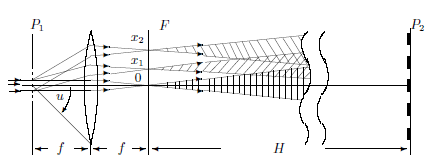
\includegraphics[width = 0.7\textwidth]{433-1.png}
			\caption{Образование изображения в объективе микроскопа.}
		\end{center}
	\end{figure}
	
	Если наблюдения ведутся при внешнем освещении, то когерентные волны рассеивают различные точки предмета. Схема образования изображения представлена на рис. 1.
	
	\subsection*{Подход Аббе к нахождению разрешающей способности микроскопа}
	Разобьем путь лучей от предмета к изображению на 2 этапа:
	\begin{enumerate}
		\item Картина, возникающая в задней фокальной плоскости $F$ --- \textit{первичное изображение}. 
		\item Первичное изображение --- источник волн $\Rightarrow$. Из этих волн возникает \textit{вторичное изображение}.
	\end{enumerate}
	
	Легко видеть, что первичное изображение представляет собой картину дифракции Фраунгофера. 
	
	\begin{figure}[h]
		\begin{center}
			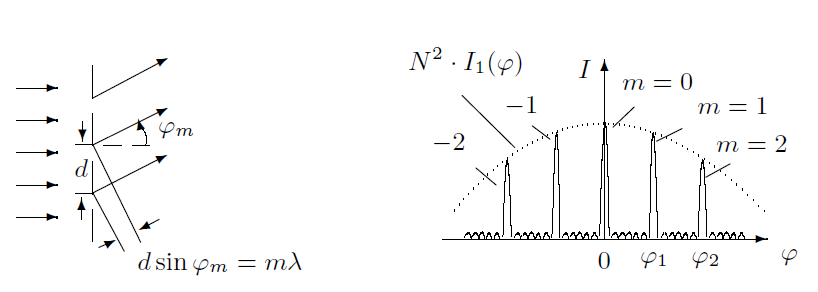
\includegraphics[width = 0.8\textwidth]{433-2.png}
			\caption{Спектр амплитудной решетки}
		\end{center}
	\end{figure}
	При дифракции Фраунгофера на решетке периода $d$ направления $\varphi_m$ максимальной интенсивности определяются из условия 
	\begin{equation}
	d \sin \varphi_m = m \lambda
	\end{equation}
	
	Из рис. 2 легко видеть, что у различных максимумов разные интенсивности.
	В итоге у нас излучение точечных источников на равном расстоянии, отсюда интерференция. 
	
	При таком рассмотрении, из того, что линза конечна следует, что есть дифракционные искажения, так как проходят только те волны, для которых верно 
	\begin{equation}
	\varphi_m < u
	\end{equation}
	
	где $u$ --- \textit{апертурный угол} (см. рис. 1).
	
	\begin{wrapfigure}{r}{0.35\textwidth}
		\begin{center}
			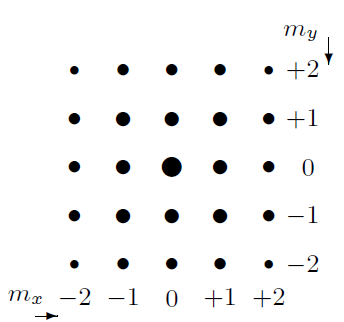
\includegraphics[width = 0.25\textwidth]{433-3.png}
		\end{center}
		\caption{Дифракция Фраунгофера на двумерной решетке}
	\end{wrapfigure}
	
	Если приоткрыть диафрагму и пустить нулевой и один из первых максимумов, то получим периодическую картинку, рассчитаем период. $x_1$ между нулевым и первыми максимумами:
	\begin{equation}
	x_1 \approx f \varphi_1 = f \lambda/d
	\end{equation} 
	
	Ширина интерференционных полос:
	\begin{equation}
	l = \lambda/\omega
	\end{equation} 
	
	где $\omega = x_1/H$ --- угол схождения интерферирующих лучей в точке наблюдения, а $H$ --- расстояние между $F$ и $P_2$. Таким образом, 
	\begin{equation}
	l \approx \lambda H/x_1 = H d/f
	\end{equation}
	
	\begin{equation}
	d' \approx \dfrac{H + f}{f} d
	\end{equation}
	
	Условие разрешения решетки с периодом $d$:
	\begin{equation}
	\sin u \geqslant \lambda/d \Rightarrow 
	\end{equation}
	
	\begin{equation}
	d \geqslant \dfrac{\lambda}{\sin u} \approx \dfrac{\lambda}{D/2f}
	\end{equation}
	Если есть не только 0 максимум, то 
	\begin{equation}
	d \geqslant \dfrac{\lambda}{2 \sin u}
	\end{equation}
	
	У нас решетка двумерная, поэтому мы можем записать все тоже самое в двух осях и получить картину как на рис. 3.
	
	
\section*{Экспериментальная установка}

Схема модели проекционного микроскопа приведена на рис. 4. Предметом служат сетки, расположенные
в кассете. Смена сеток осуществляется поворотом внешнего кольца кассеты.

    \begin{figure}[h]
    \centering
    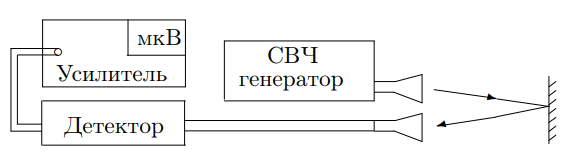
\includegraphics[width=15cm]{fig1.PNG}
    \caption{Схема экспериментальной установки — модель проекционного
микроскопа}
    \label{fig:vac}
\end{figure}


\newpage
\section*{{Выполнение работы}}
\subsection*{Определение периода решёток по их пространственному спектру}
    Для определения периода решёток $d$ измерим расстояния $l$ между максимумами разных порядков $n$ на экране. Расстояние от сетки до экрана $D = 138 $ см. Период решётки рассчитывается по формуле: 
    \begin{equation*}
        d = \frac{\lambda D}{x}, 
    \end{equation*}
    где $x$ - расстояние между соседними максимумами.\\
    Результаты измерений занесём в таблицу 1.
    
\begin{table}[h!]
  \centering
    \begin{center}
    \caption{Периоды решёток с помощью метода пространственного спектра}
    \end{center}
\begin{tabular}{|c|c|c|c|c|c|c|c|c|}
\hline
N сетки & n, ед & $\sigma_{n}$, ед        & x,мм & $\sigma_{x}$, мм        & D, мм                 & $\sigma_{D}$, мм        & d, мкм & $\sigma_{d}$, мкм \\ \hline
1       & 2     & \multirow{5}{*}{1} & 76   & \multirow{5}{*}{2} & \multirow{5}{*}{1380} & \multirow{5}{*}{2} & 19     & 3            \\ \cline{1-2} \cline{4-4} \cline{8-9} 
2       & 2     &                    & 51   &                    &                       &                    & 29     & 3            \\ \cline{1-2} \cline{4-4} \cline{8-9} 
3       & 3     &                    & 39   &                    &                       &                    & 56     & 3            \\ \cline{1-2} \cline{4-4} \cline{8-9} 
4       & 8     &                    & 50   &                    &                       &                    & 117    & 3            \\ \cline{1-2} \cline{4-4} \cline{8-9} 
5       & 13    &                    & 61   &                    &                       &                    & 156    & 4            \\ \hline
\end{tabular}
\end{table}
Погрешность $d$ считаем по формуле:
$$
\sigma_{d} = \sqrt{\left(\dfrac{\partial d}{\partial  x}\right)^2 \sigma^2_{x} + \left(\dfrac{\partial d}{\partial n}\right)^2 \sigma^2_{n} + \left(\dfrac{\partial d}{\partial \Delta x}\right)^2 \sigma^2_{D}} =\lambda \sqrt{\dfrac{n^2 D^2 \sigma^2_{x}}{x^4} + \dfrac{x^2 \sigma^2_{n} \sigma^2_{D}}{n^2} + \dfrac{D^2 \sigma^2_{n}}{x^2}}.
$$

\subsection*{Определение периода решёток по изображению, увеличенному
с помощью модели микроскопа}
    Соберём модель проекционного микроскопа (рис. 4), отцентрируем систему. Измеряем необходимые расстояния:
$$
\begin{array}{r}
a_1 = 120 \pm 10 \text{ мм},\\
a_2 + b_1 = 455 \pm 10 \text{  см},\\
b_2 = 815 \pm 10 \text{ см},
\end{array}
$$
Погрешности здесь обусловлены неточностями в положенияъ сеток и линз. Из формулы тонкой линзы $a_2 = \frac{b_2 F_2}{b_2 - F_2} = 25.79 \text{ мм}$, откуда $a_2 \approx F_2$, поэтому в дальнейшем будем использовать это значение, следовательно $b_1 = 420 \pm 10 \text{ мм}$. \\
Увеличение микроскопа $\Gamma = \dfrac{b_1 b_2}{a_1 a_2} = 114 \pm 10$. Погрешность $\Gamma$ находится по формуле:
$$
\sigma_\Gamma = \sqrt{\left(\dfrac{\partial \Gamma}{\partial a_1}\right)^2 \sigma^2_{a_1} + \left(\dfrac{\partial \Gamma}{\partial b_1}\right)^2 \sigma^2_{b_1} + \left(\dfrac{\partial \Gamma}{\partial b_2}\right)^2 \sigma^2_{b_2}}.
$$
    На экране измерим расстояния между максимумами разных порядков. Результаты измерений занесём в таблицу 2.
\begin{table}[h!]
  \centering
    \begin{center}
    \caption{Периоды решёток по изображению микроскопа}
    \end{center}
\begin{tabular}{|c|c|c|c|c|c|c|c|}
\hline
N сетки & $\Delta x$,мм & $\sigma_{\Delta x}$,   мм & n  & $\Gamma$               & $\sigma_\Gamma$         & d, мкм & $\sigma_{d}$, мкм \\ \hline
1       & 37         & \multirow{5}{*}{2}   & 16 & \multirow{5}{*}{114} & \multirow{5}{*}{10} & 20     & 2            \\ \cline{1-2} \cline{4-4} \cline{7-8} 
2       & 157        &                      & 49 &                      &                     & 28     & 3            \\ \cline{1-2} \cline{4-4} \cline{7-8} 
3       & 253        &                      & 38 &                      &                     & 58     & 5            \\ \cline{1-2} \cline{4-4} \cline{7-8} 
4       & 241        &                      & 18 &                      &                     & 117    & 12           \\ \cline{1-2} \cline{4-4} \cline{7-8} 
5       & 236        &                      & 13 &                      &                     & 159    & 19           \\ \hline
\end{tabular}
\end{table}    

Здесь $d$ определялось по формуле $d = \dfrac{\Delta x}{\Gamma n}$, погрешность
$$
\sigma_d = \sqrt{\left(\dfrac{\partial d}{\partial \Delta x}\right)^2 \sigma^2_{\Delta x} + \left(\dfrac{\partial d}{\partial n}\right)^2 \sigma^2_{n} + \left(\dfrac{\partial d}{\partial \Gamma}\right)^2 \sigma^2_{\Gamma}}.
$$

Важно отметить, что значения периодов решеток, измеренные двумя вышеприведенными способами, совпадают в пределах погрешности.

\subsection*{Определение периода решёток по оценке разрешающей способности микроскопа}
Поместим в фокальной плоскости линзы $\text{Л}_1$ щелевую диафрагму с микрометрическим винтом и определим минимальную толщину $D$ при которой на экране видна двумерная решётка. В этом случае период будет вычисляться в предельном случае по формуле:
$$
d = \dfrac{2\lambda F_1}{D},
$$
погрешность вычисляется по формуле 
$$
\sigma_d = d \dfrac{\sigma_D}{D}.
$$
Результаты приведены в Таблице 3.
\begin{table}[h]
\begin{tabular}{|c|c|c|c|}
\hline
D, мм & $\sigma_D$, мм & $d$, мкм & $\sigma_d$, мкм \\ \hline
4.14  & 0.02           & 28.27    & 3            \\ \hline
1.960 & 0.010          & 59.7     & 3             \\ \hline
1.020 & 0.010          & 114.7    & 3             \\ \hline
0.810 & 0.010          & 144.5    & 4             \\ \hline
\end{tabular}
\centering
\caption{Периоды решёток, метод 3.}
\end{table}\\
Через щель проходили только нулевой (по центру) и два первых максимумы, за исключением второй щели, где нулевой максимум был помещён к краю щели. Для первой решётки период таким методом измерить не получилось, так как ширины щели не хватает.
\newpage
\begin{figure}[h]
\includegraphics[scale=0.7]{2.png}
\centering
\caption{Зависимость $d = f(1/D)$.}
\end{figure}
Для проверки теории Аббе построим график $d = f(\frac{1}{D})$ со значениями $d$ из части 3.
Найдем коэффициент наклона касательной:
\begin{equation*}
    k = \sqrt{\frac{<xy>-<x>\cdot<y>}{<x^2>-<x>}}
\end{equation*}
\begin{equation*}
    \sigma_k = \sqrt{\frac{1}{n-1}(\frac{<y^2>}{<x^2>}-k^2)}
\end{equation*}
$k = (124 \pm 8) \cdot 10^{-9} \text{ м}^2$, в пределах погрешности он совпадает с теоретическим $2\lambda F_1 = 117 \cdot 10^{-9} \text{ м}^2$. Таким образом, теория Аббе подтвердилась.
\begin{table}[h]
\begin{tabular}{|c|c|c|c|c|}
\hline
Реш. & $1/D$, $\text{мм}^1$ & $\sigma_{1/D}$, $\text{мм}^1$ & $d$, мкм & $\sigma_d$, мкм \\ \hline
2    & 0.2415               & 0.0012                        & 30       & 3               \\ \hline
3    & 0.510                & 0.003                         & 60       & 3               \\ \hline
4    & 0.980                & 0.010                         & 117      & 3               \\ \hline
5    & 1.235                & 0.015                         & 159      & 4               \\ \hline
\end{tabular}
\centering
\caption{Значения для графика $d = f(1/D)$.}
\end{table}
\newpage
\subsection*{ Пространственная фильтрация и мультиплицирование}
Для наблюдения фильтрации на сетке 2 откроем щель так, чтобы она пропускала только максимум нулевого порядка и, поворачивая щель, наблюдаем за изменением картины. Картины представлены на Рис 6.
\begin{figure}[h]
\includegraphics[scale=0.5]{3.png}
\centering
\caption{Слева направо: горизонтальная щель $(0,m_y)$, щель на $45^\circ$ ($m_x = m_y$), вертикальная щель $(m_x,0)$.}
\end{figure}\\
Для наблюдения мультиплицирования поменяем местами сетку и щель, пронаблюдаем мультипликацию, картина представлена на Рис. 7.
\begin{figure}[h]
\includegraphics[scale=0.7]{4.png}
\centering
\caption{Явление мультипликации.}
\end{figure}
\section*{Вывод}
В ходе работы были измерены периоды различных дифракционных решёток тремя различными способами: по пространственному спектру, изображению с микроскопа и по оценке разрешающей способности микроскопа. Результаты измерений практически совпадают. Сравнение результатов, полученных разными методами, приведено в таблице 5. 

Также в работе наблюдалось и объяснялось явление пространственной фильтрации и мультиплицирования. Фактически проводилась работа с фурье-образами щели и сетки, то есть выделение и рассечение образа.

     \begin{table}[h!]
    \centering
    \begin{center}
    \caption{Периоды решёток, различные методы}
    \end{center}
    \vspace{0.1cm}
    \label{tab:my_label}
    \begin{tabular}{ |p{4cm}||p{1.2cm}|p{1.2cm}|p{1.2cm}|p{1.2cm}|p{1.3cm}|}
 \hline
Номер решётки & 1 & 2 & 3 & 4 & 5\\
 \hline
 $d$, мкм - простр. спектр  & 19\pm 3 & 29\pm 3 & 56\pm 3 & 117\pm 3 & 156\pm 4 \\
 \hline
 $d$, мкм - микроскоп & 20\pm 2 & 28\pm 3 & 58\pm 5 & 117\pm 12 & 159\pm 19 \\
 \hline
 $d$, мкм - диафрагма  & - & 30\pm 3 & 60\pm 3 & 117\pm 3 & 159\pm 4 \\

 \hline
 
\end{tabular}
\end{table}   


\end{document}
